\chapter{Additional Figures}
\label{ch:additional-materials}

The following figures are listed in this section:

\begin{itemize}[leftmargin=0mm]
\item \textbf{\cref{fig:additional:tdm-causal-factors} (p\pageref{fig:additional:tdm-causal-factors})}
  highlights potential causal factors that may influence a developer's understanding of the documentation and response of \glspl{iws}. It was intended to be used as the basis of a survey study in \cref{ch:tse2020}, and can be used for future avenues of research.
\item \textbf{\cref{fig:additional:propsed-tdm} (p\pageref{fig:additional:propsed-tdm})}
  was intended for the discussion in \cref{ch:icse2020}, where we propose that developers have a misaligned of the technical domain models within \glspl{iws} and more specifically \glspl{cvs}. We designed a draft technical domain model to describe the various aspects developers must consider when using these services, based on the work by \citet{Barnett:2018Kx}. 
\item \textbf{\cref{fig:additional:tdm-questions} (p\pageref{fig:additional:tdm-questions})}
  describes potential questions that may arise to analyse and test the causal factors of the technical domain model proposed in \cref{fig:additional:propsed-tdm}. This lies an open avenue of future research.
\item \textbf{\cref{fig:additional:threshy-decision-boundary} (p\pageref{fig:additional:threshy-decision-boundary})}
  emphasises dichotomy between an application using an \gls{iws} and the \gls{iws}' training data (which is sourced from an unknown context) and the context of an application, which is known. This is to emphasise how the model produced from these services need to be calibrated to the application domain being used in order for the decision boundary of a single inference to be properly assessed by the developer. This image was originally included within the Threshy publication (\cref{ch:fse-demo2020}) but was removed due to space limitations.
\item \textbf{\cref{fig:additional:threshy-domain-model} (p\pageref{fig:additional:threshy-domain-model})}
  illustrates the domain model of Threshy (\cref{ch:fse-demo2020}).
\item \textbf{\cref{fig:additional:threshy-sequence-diagram} (p\pageref{fig:additional:threshy-sequence-diagram})}
  illustrates the dynamic model of using Threshy and its interactions between the application, front-end of Threshy and back-end of Threshy (\cref{ch:fse-demo2020}).
\item \textbf{\cref{fig:additional:so-post-extension} (p\pageref{fig:additional:so-post-extension})}
  was originally included within the publication \cref{ch:icse2020} but was removed due to space limitations. It provides a high-level overview of the main steps we performed within this study.
\item \textbf{\cref{fig:additional:arch-class-diagram} (p\pageref{fig:additional:arch-class-diagram})}
  is a class diagram of the reference architecture of the proposed architecture in \cref{ch:fse2020}. The implementation is provided in \cref{ch:reference-architecture-code}. See \cref{ch:fse2020} for more.
\item \textbf{\cref{fig:additional:arch-create-new-brc} (p\pageref{fig:additional:arch-create-new-brc})}
  is a sequence diagram illustrating how the reference architecture can be used to create a new benchmark as per the implementation provided in \cref{ch:reference-architecture-code}. See \cref{ch:fse2020} for more.
\item \textbf{\cref{fig:additional:arch-make-request} (p\pageref{fig:additional:arch-make-request})}
  is a sequence diagram illustrating how applications can make requests to the proxy server `facade' as per the implementation provided in \cref{ch:reference-architecture-code}. See \cref{ch:fse2020} for more.
\item \textbf{\cref{fig:additional:arch-overall-state} (p\pageref{fig:additional:arch-overall-state})}
  is a state diagram that illustrates the overall states that exist within the architecture tactic's workflows. See \cref{ch:fse2020} for more.
\item \textbf{\cref{fig:additional:arch-evolution-of-brc} (p\pageref{fig:additional:arch-evolution-of-brc})}
  is a sequence diagram illustrating how the reference architecture handles evolution in an external service per the implementation provided in \cref{ch:reference-architecture-code}. See \cref{ch:fse2020} for more.
\item \textbf{\cref{fig:additional:arch-evolution-dynamic} (p\pageref{fig:additional:arch-evolution-dynamic})}
  illustrates how the reference architecture is able to capture and handle three requests (two valid, one invalid) when sent to the proxy server. See \cref{ch:fse2020} for more.
\end{itemize}

\begin{landscape}
\begin{figure}[p!]
\centering
\caption[Causal factors that may influence understanding of intelligent web services]{Causal factors that may influence understanding of intelligent web services.}
\label{fig:additional:tdm-causal-factors}
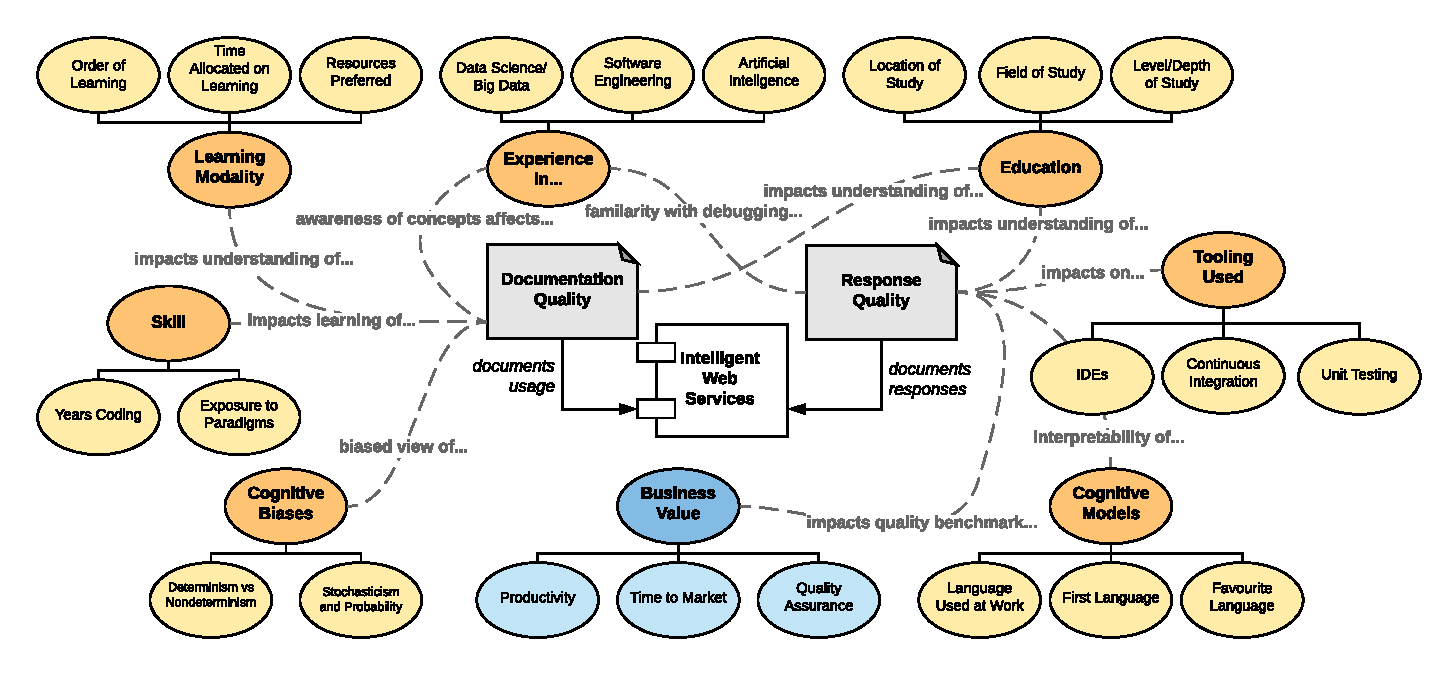
\includegraphics[width=\linewidth]{appendix/figures/tdm-causal-factors}
\end{figure}

\begin{figure}[p!]
\centering
\caption[A proposal technical domain model for intelligent services]{A proposal technical domain model for intelligent services. (The \faInfoCircle{} symbol indicates computer vision related services only.)}
\label{fig:additional:propsed-tdm}
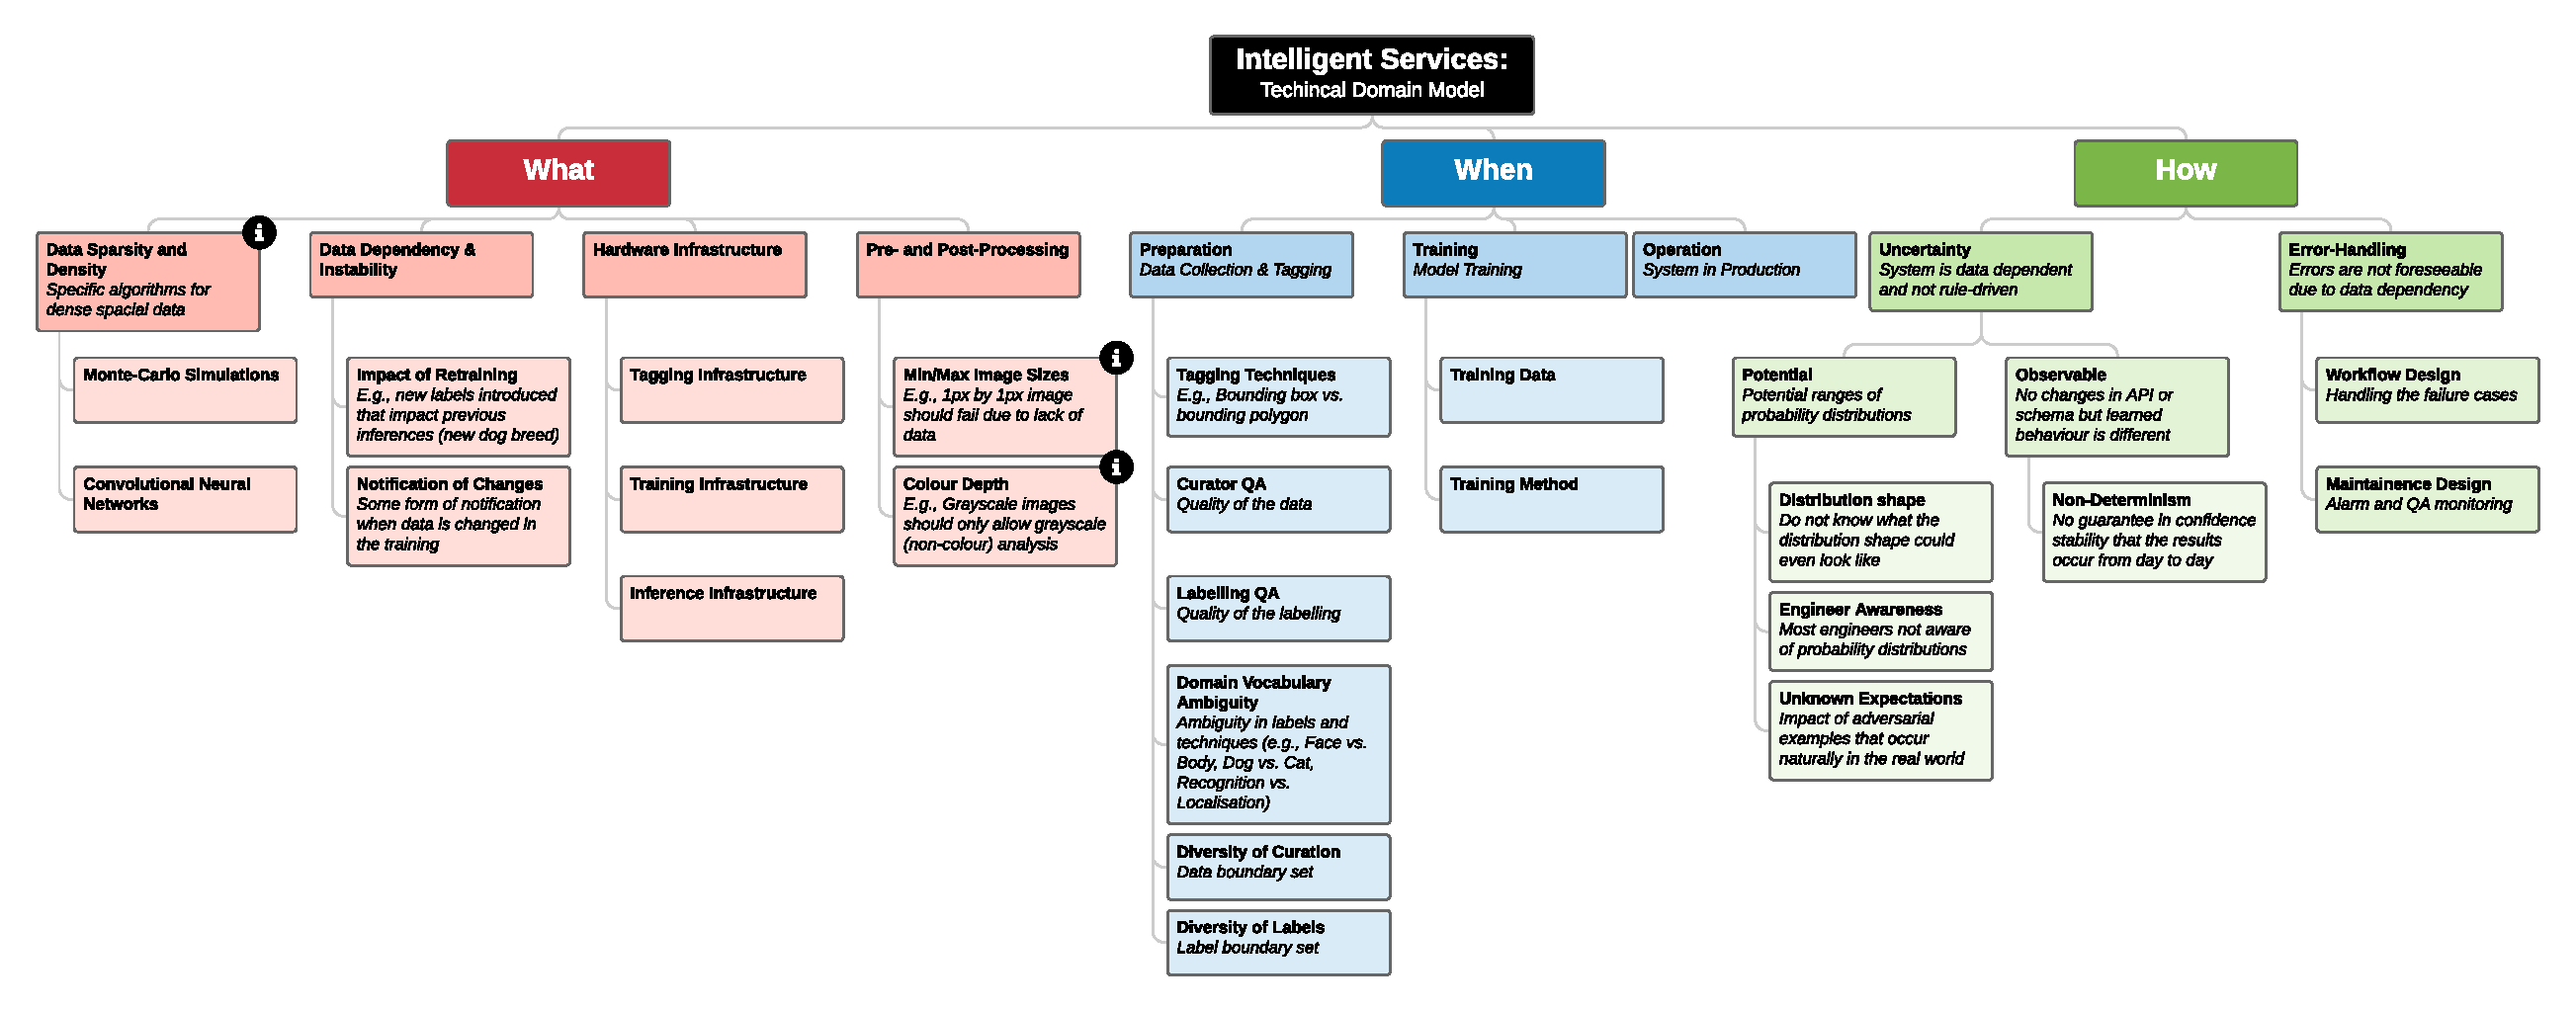
\includegraphics[width=\linewidth]{appendix/figures/proposed-tdm}
\end{figure}
\end{landscape}

\begin{figure}[p!]
\centering
\caption[Potential questions that can be asked around causal factors of a developer's understanding of an intelligent service]{Potential questions that can be asked around causal factors of a developer's understanding of an intelligent service.}
\label{fig:additional:tdm-questions}
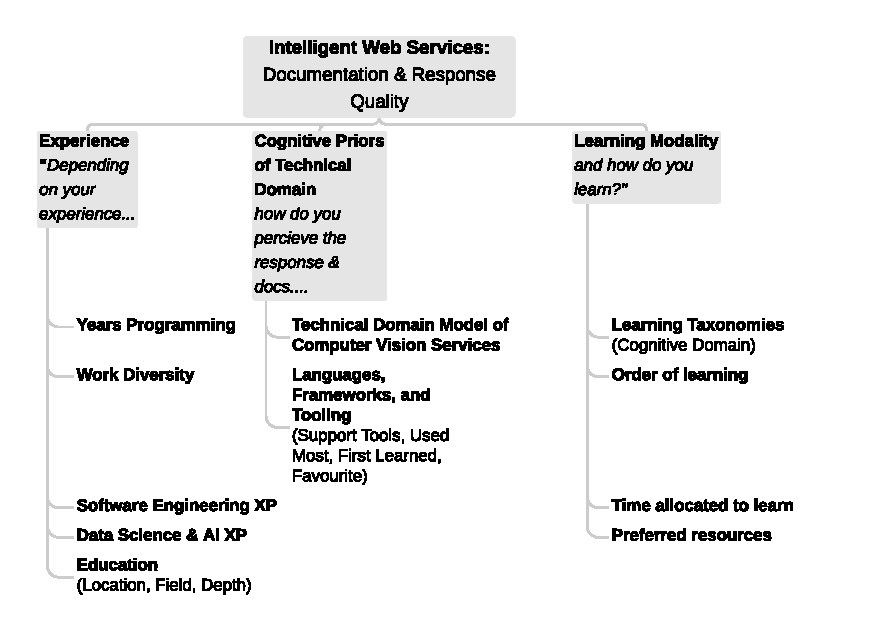
\includegraphics[width=\linewidth]{appendix/figures/tdm-questions}
\end{figure}

\begin{figure}[p!]
\centering
\caption[Threshy and developer interaction with decision boundaries]{Threshy assists with making appropriate decision boundaries in the application context by calibrating model (train on an unknown context) to your domain.}
\label{fig:additional:threshy-decision-boundary}
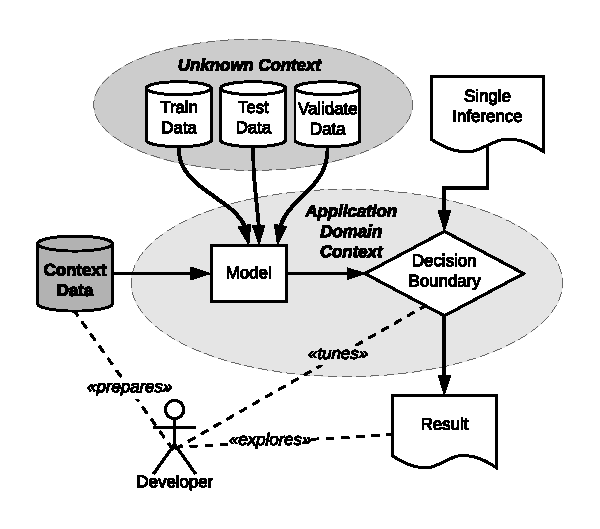
\includegraphics[width=.8\linewidth]{appendix/figures/threshy-decision-boundary}
\end{figure}

\begin{figure}[p!]
\centering
\caption[Threshy domain model]{Threshy domain model.}
\label{fig:additional:threshy-domain-model}
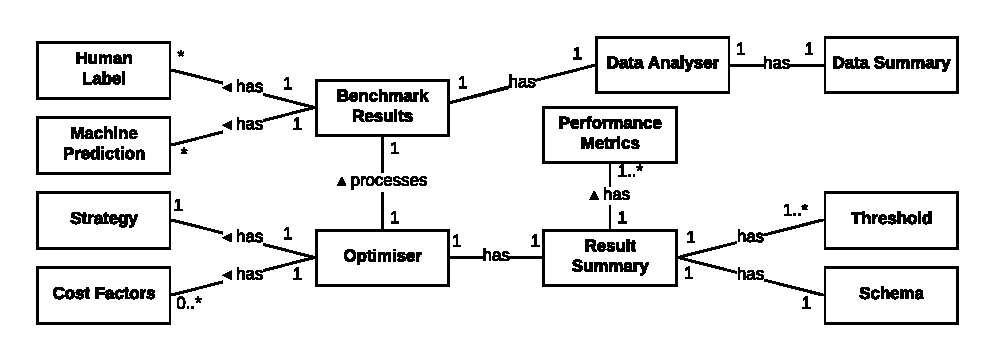
\includegraphics[width=\linewidth]{appendix/figures/threshy-domain-model}
\end{figure}

\begin{figure}[p!]
\centering
\caption[Threshy sequence diagram]{High level overview of Threshy's interaction between the front- and back-end.}
\label{fig:additional:threshy-sequence-diagram}
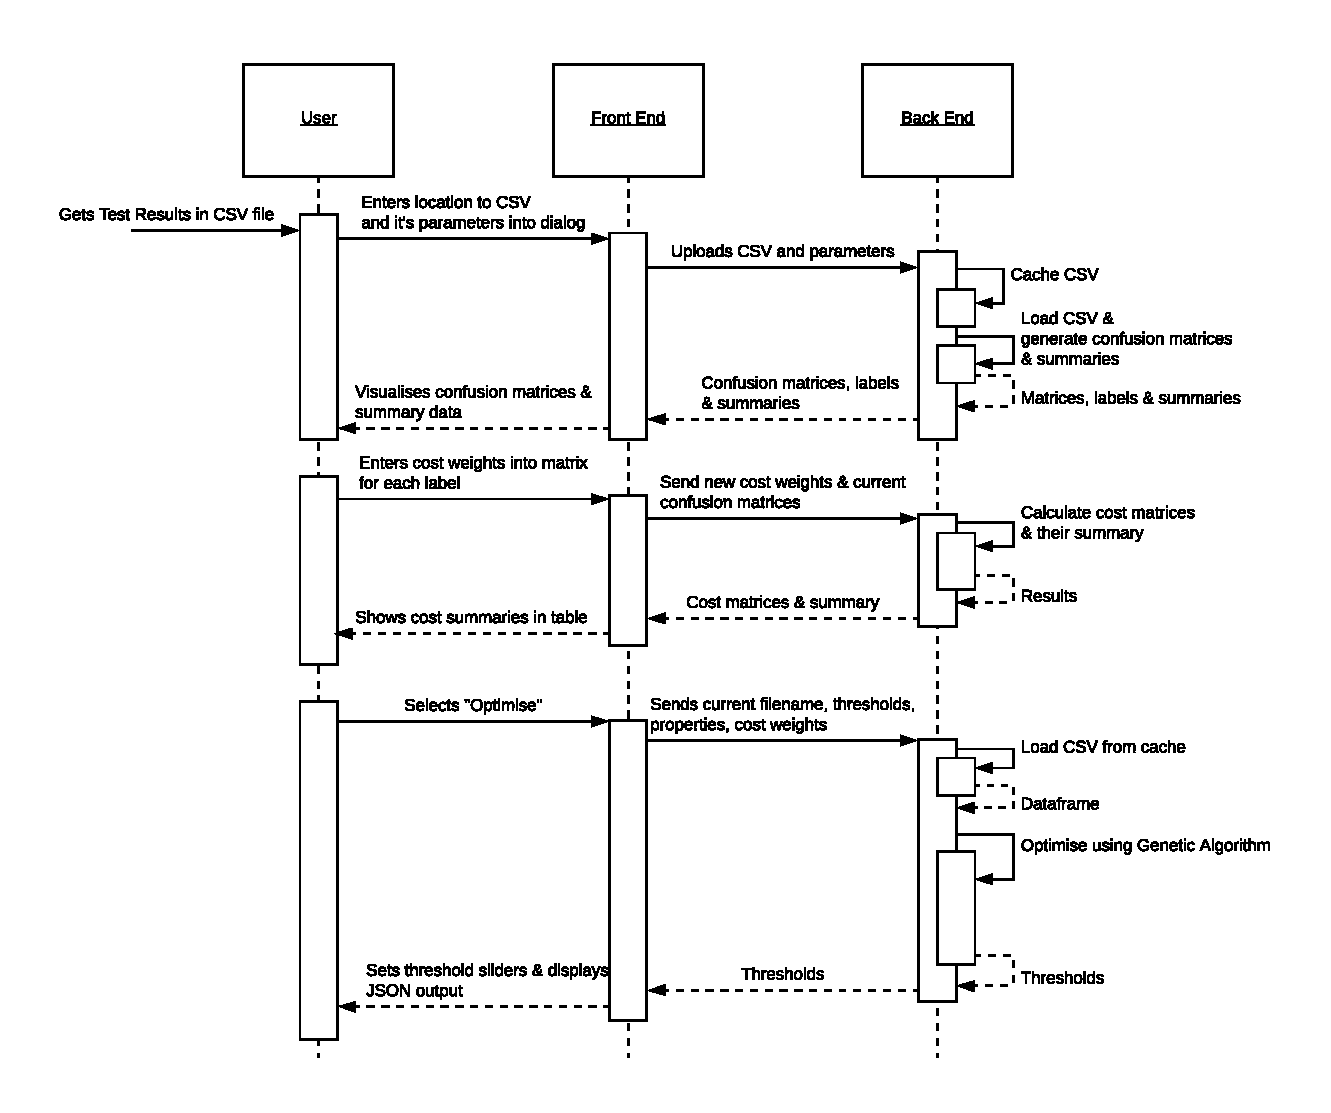
\includegraphics[width=\linewidth]{appendix/figures/threshy-sequence-diagram}
\end{figure}



\afterpage{
\begin{landscape}

\begin{figure}[p!]
\centering
\caption[High-level overview of our method in \cref{ch:icse2020}]{High-level overview of the methodology within \cref{ch:icse2020}.}
\label{fig:additional:so-post-extension}
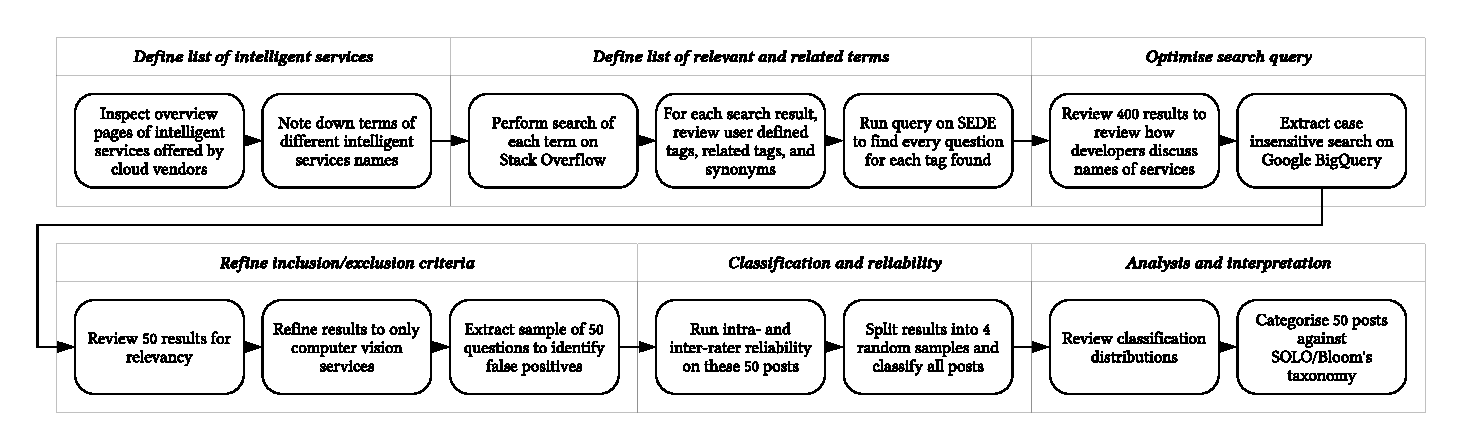
\includegraphics[width=\linewidth]{appendix/figures/so-post-extension}
\end{figure}

\begin{figure}[p!]
\centering
\caption[Class diagram of architecture implementation]{Class diagram of the implementation of our architecture.}
\label{fig:additional:arch-class-diagram}
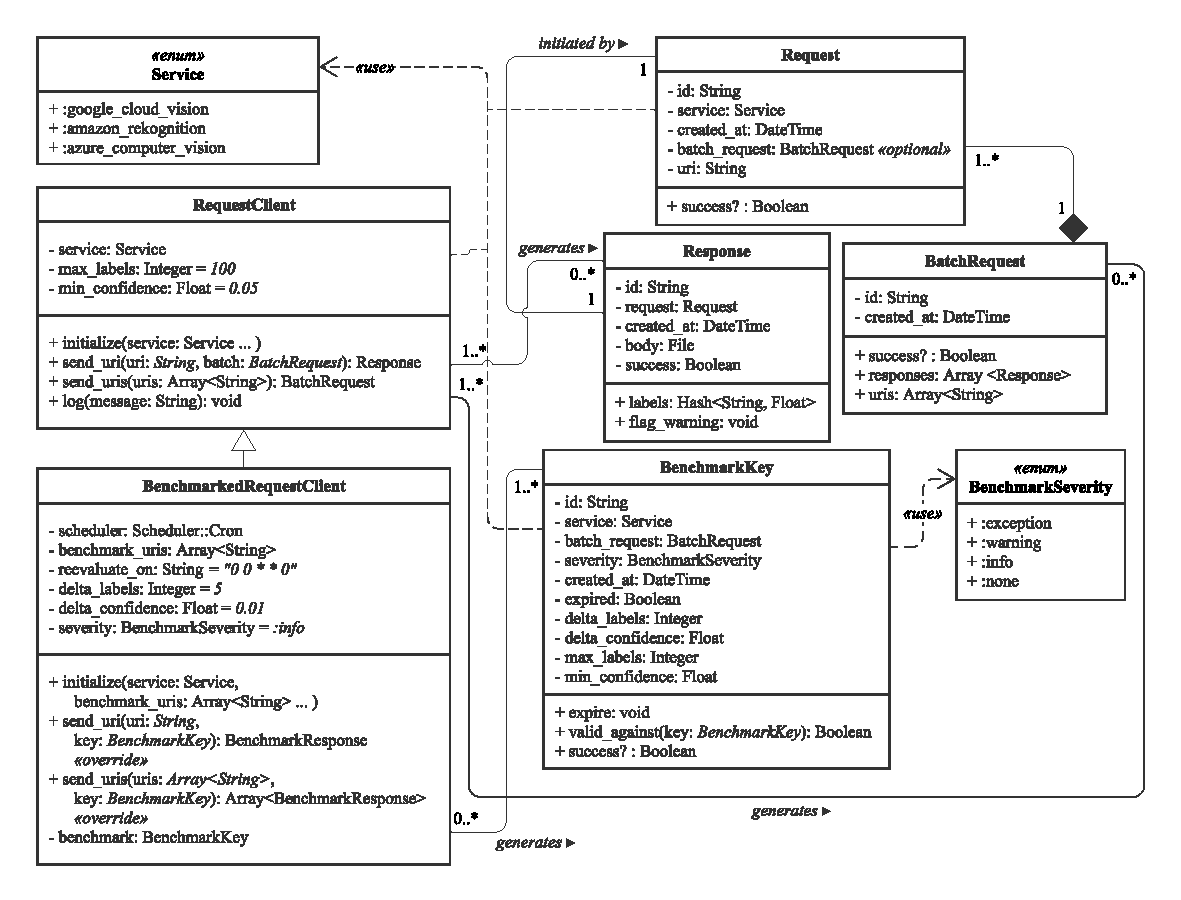
\includegraphics[width=.8\linewidth,height=\paperheight,keepaspectratio]{appendix/figures/arch-class-diagram}
\end{figure}

\begin{figure}[p!]
\centering
\caption[Creation of a benchmark using the architecture tactic]{Creation of a new benchmark proxy server using the architecture tactic.}
\label{fig:additional:arch-create-new-brc}
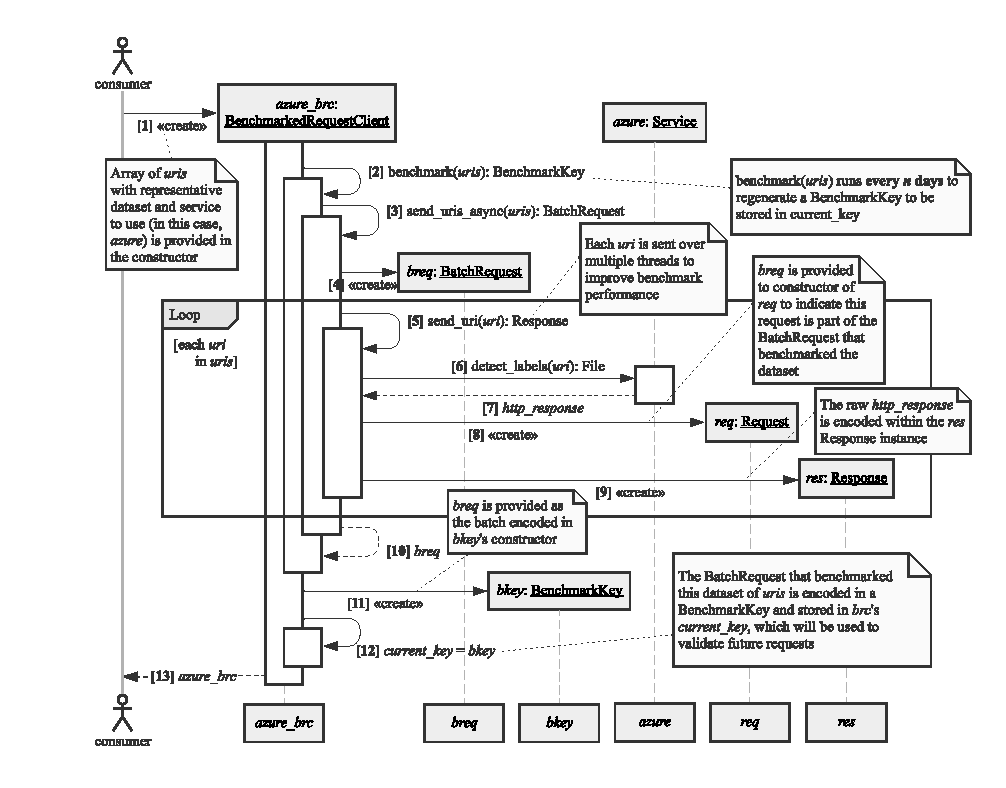
\includegraphics[width=.8\linewidth,height=\paperheight,keepaspectratio]{appendix/figures/arch-create-new-brc}
\end{figure}

\begin{figure}[p!]
\centering
\caption[Making a request via the proxy server facade]{Making a request through the proxy server `facade'.}
\label{fig:additional:arch-make-request}
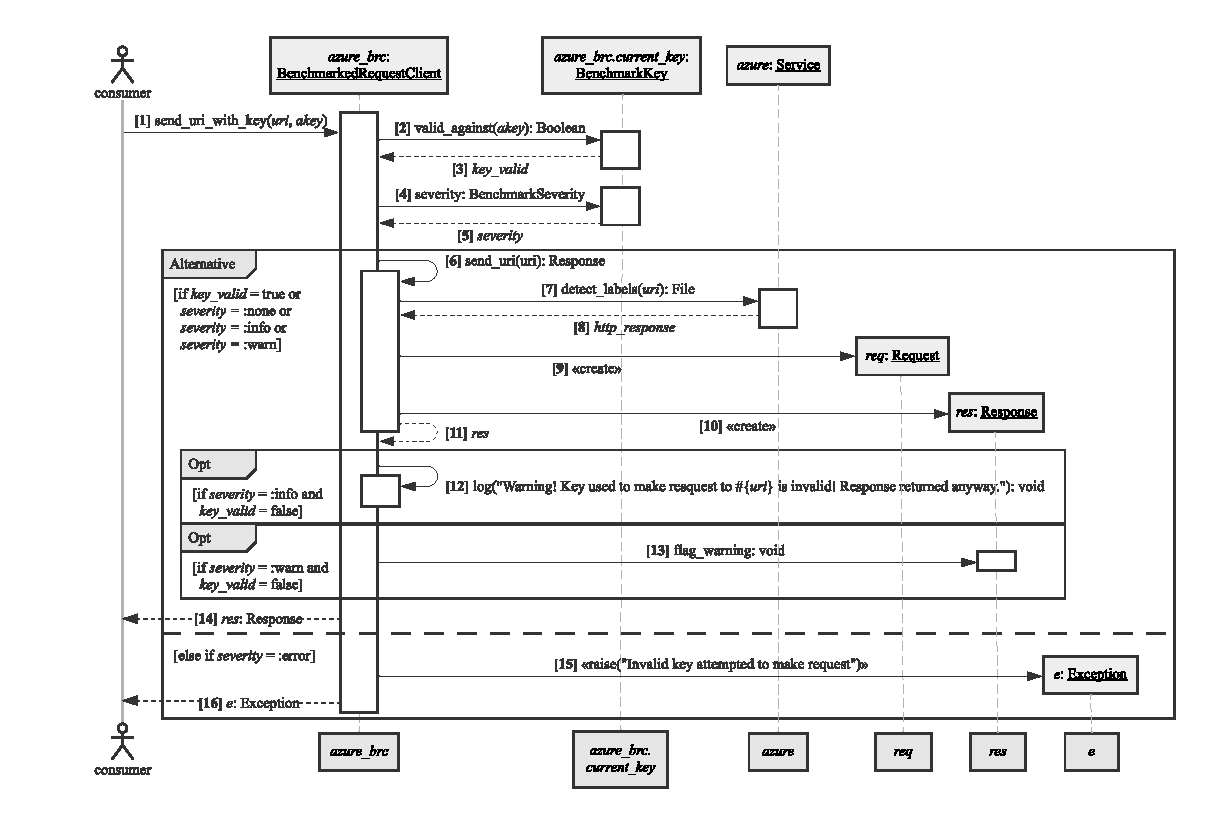
\includegraphics[width=.9\linewidth,height=\paperheight,keepaspectratio]{appendix/figures/arch-make-request}
\end{figure}

\begin{figure}[p!]
\centering
\caption[High-level workflow of the architectural tactic]{State diagram of high-level workflows in the architectural tactic.}
\label{fig:additional:arch-overall-state}
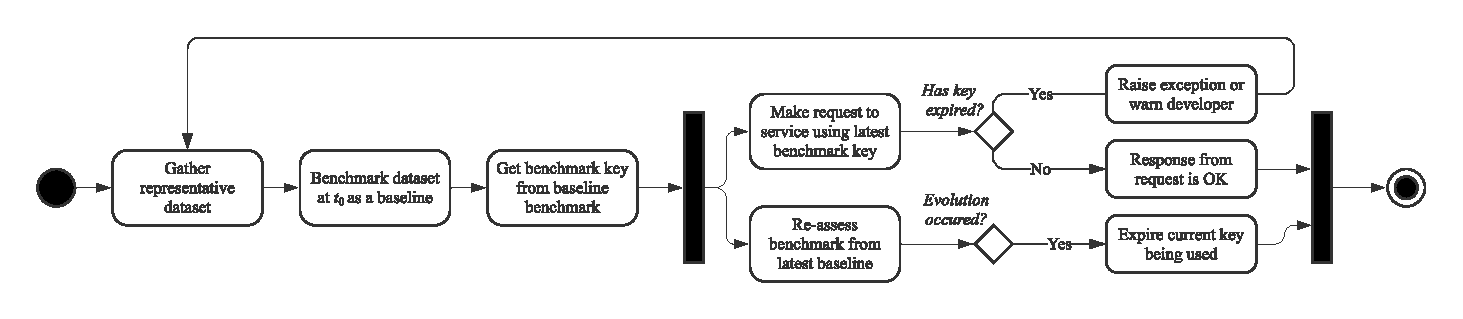
\includegraphics[width=\linewidth]{appendix/figures/arch-overall-state}
\end{figure}

\begin{figure}[p!]
\centering
\caption[Handling of evolution using our architecture (i)]{Evolution occurring in the benchmark and how the architectural tactic notifies the consumer.}
\label{fig:additional:arch-evolution-of-brc}
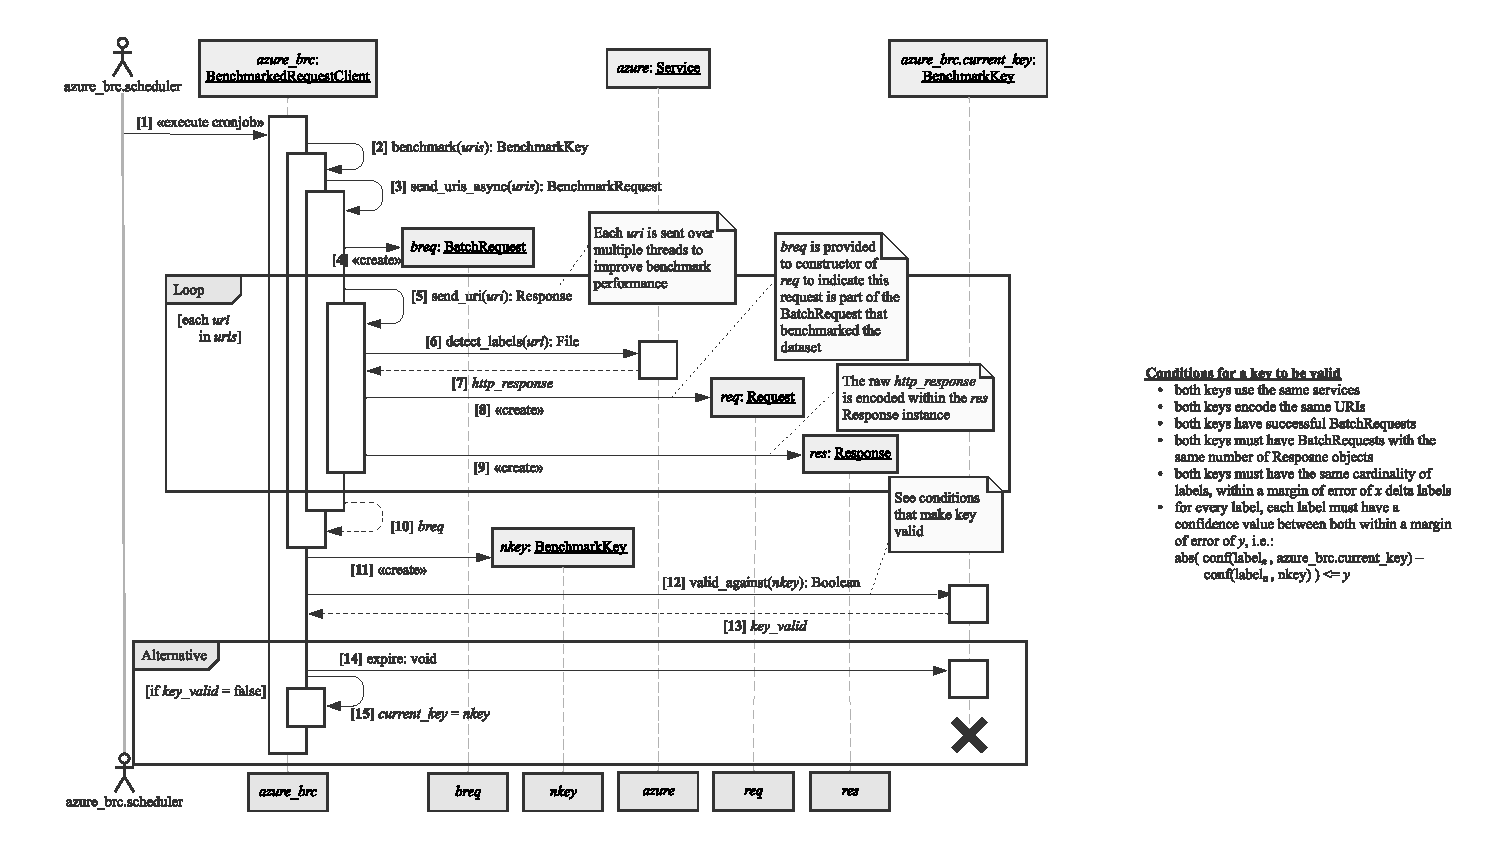
\includegraphics[width=\linewidth,height=\paperheight,keepaspectratio]{appendix/figures/arch-evolution-of-brc}
\end{figure}


\begin{figure}[p!]
\centering
\caption[Handling of evolution using our architecture (ii)]{Evolution occurring in an intelligent service and how the architectural tactic handles it.}
\label{fig:additional:arch-evolution-dynamic}
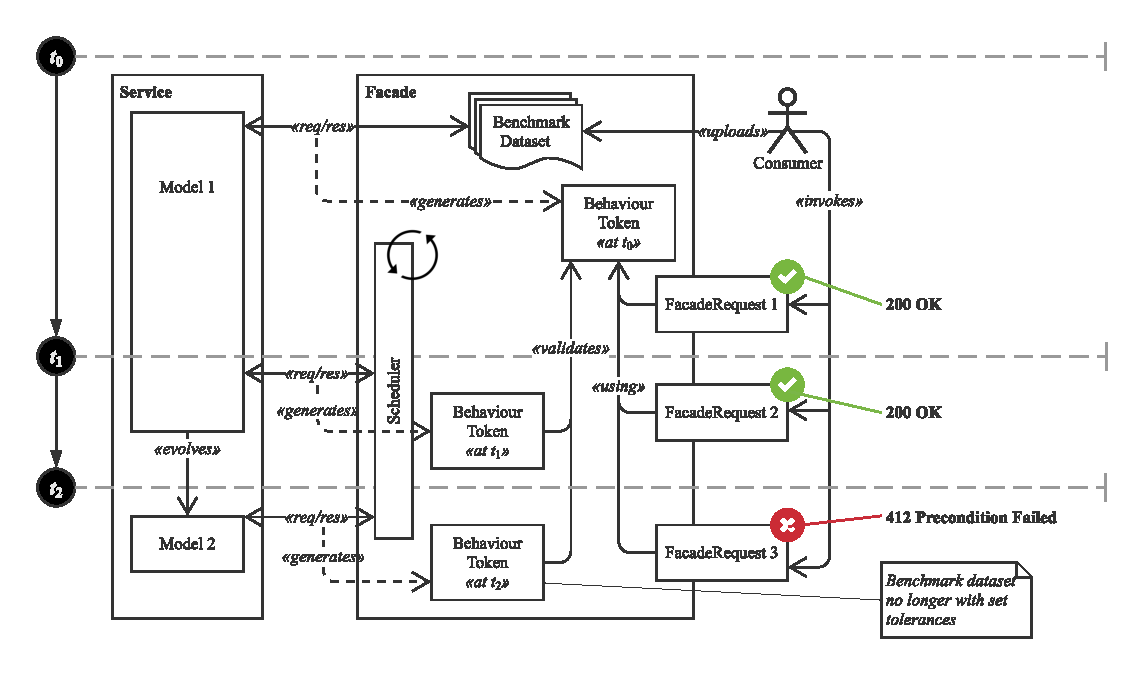
\includegraphics[width=.9\linewidth,height=\paperheight,keepaspectratio]{appendix/figures/arch-evolution-dynamic}
\end{figure}



\end{landscape}}

\clearpage

\chapter{Reference Architecture Source Code}
\label{ch:reference-architecture-code}

% Include ICVS Benchmarker Facade Code...
\lstinputlisting[basicstyle=\ttfamily\scriptsize,language=ruby,caption={[Implementation of the architecture module components]{Implementation of architecture module components.}}]{appendix/code/icvsb.rb}
\clearpage
\lstinputlisting[basicstyle=\ttfamily\scriptsize,language=ruby,caption={[Implementation of the architecture facade API]{Implementation of the architecture facade API.}}]{appendix/code/server.rb}